\documentclass[tikz]{standalone}
\usepackage{amsmath}
\usetikzlibrary{calc}
\begin{document}
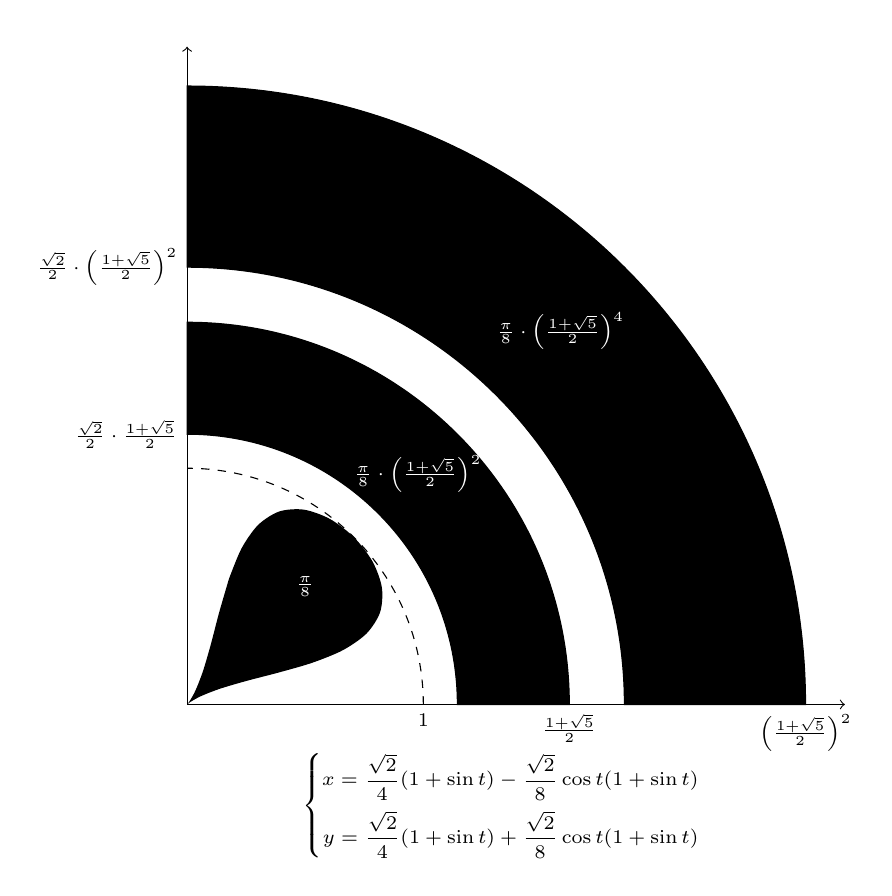
\begin{tikzpicture}

    \pgfmathsetmacro\gr{(1+sqrt(5))/2}
    \pgfmathsetmacro\u{3}
    \pgfmathsetmacro\rao{\u*\gr*\gr}
    \pgfmathsetmacro\rbo{\u*\gr}
    \pgfmathsetmacro\rco{\u}
    \pgfmathsetmacro\a{\rco/2}
    \newcommand{\makeb}[1]{#1/2}
    \pgfmathsetmacro\PI{3.1415926}
    \pgfmathsetmacro\area{\PI*\a*\makeb{\a}}
    \pgfmathsetmacro\rai{sqrt(pow(\rao,2)-4*pow(\gr,4)*\area/\PI)}
    \pgfmathsetmacro\rbi{sqrt(pow(\rbo,2)-4*pow(\gr,2)*\area/\PI)}
    \newcommand{\px}[2]{#2*(1+sin(#1))}
    \newcommand{\py}[2]{\makeb{#2}*cos(#1)*(1+sin(#1))}
    \newcommand{\rpx}[2]{cos(45)*\px{#1}{#2}-sin(45)*\py{#1}{#2}}
    \newcommand{\rpy}[2]{sin(45)*\px{#1}{#2}+cos(45)*\py{#1}{#2}}
    \newcommand{\cc}[5]{
        \draw[fill=black]
        ($(c1) + (0:#2)$) arc (0:90:#2)
        --
        ($(c1) + (90:#1)$) arc (90:0:#1)
        -- cycle;
        \node[left] at (0,#1) {\scriptsize $#3$};
        \node[below] at (#2,0) {\scriptsize $#4$};
        \pgfmathsetmacro\p{(#1+#2)/2/sqrt(2)};
        \node[color=white] at (\p,\p) {\scriptsize $#5$};
    }
    \newcommand{\gra}{\ensuremath{\frac{1+\sqrt{5}}{2}}}
    \newcommand{\grb}{\ensuremath{\left(\gra\right)^2}}
    \newcommand{\grd}{\ensuremath{\left(\gra\right)^4}}
    \newcommand{\tot}{\ensuremath{\frac{\sqrt{2}}{2}}}

    \coordinate (c1) at (0, 0);
    \cc{\rbi}{\rbo}{\tot\cdot\gra}{\gra}{\frac{\pi}{8}\cdot\grb}
    \cc{\rai}{\rao}{\tot\cdot\grb}{\grb}{\frac{\pi}{8}\cdot\grd}
    \fill [black,domain=0:360] plot[smooth] ({\rpx{\x}{\rco/2}}, {\rpy{\x}{\rco/2}});
    \pgfmathsetmacro\p{\u/2}
    \node[color=white] at (\p,\p) {\scriptsize $\frac{\pi}{8}$};
    
    \draw[->] (0,0) -- (\rao+0.5,0) node[right] {};
    \draw[->] (0,0) -- (0,\rao+0.5) node[above] {};
    \draw[dashed] ($(c1) + (0:\rco)$) arc (0:90:\rco);
    \node[below] at (\u,0) {\scriptsize $1$};
    \node[below] at (4,-0.5) {\scriptsize%
        $\left\{\begin{aligned}
            x = \frac{\sqrt{2}}{4}(1+\sin t) - \frac{\sqrt{2}}{8}\cos t(1+\sin t) \\
            y = \frac{\sqrt{2}}{4}(1+\sin t) + \frac{\sqrt{2}}{8}\cos t(1+\sin t) \\
        \end{aligned}\right.$%
    };

\end{tikzpicture} 
\end{document}
